% H08: context is the coupling. Sources: hypotheses/H08-context-is-the-coupling/{README.md (Round 1b), summary/content.tex, summary/meta.json};
% writeup/visuals/H08-context-is-the-coupling/{caption.tex, README.md}; interpretation/swarm-constants.json (t_read).
\section{H08: A message acts only at the call that receives it}

\textbf{The question:}
Do agents couple only through what enters their model calls?
If so, a message cannot change an agent until a call has the message in its context.
The coupling delay then equals the call cadence, not the time the message sits in the room.

\textbf{The intuition:}
Model 02 gives each agent two variables.
The visible spin is what the agent does; the hidden field is the set of room messages that arrived since its last call.
The scaffold builds the context at the start of each call, and the call reads and clears the hidden field.
The couplings $J_{ij}$, the effect of agent $j$'s messages on agent $i$, act only at that moment.
Think of an information channel that opens once per call.
The prediction is a jump in response at call offset 1, the receiving call.
At offset 0, the call already in flight, the response stays at zero.
A common cause, where both agents react to one earlier event, gives a flat floor, not a jump.

\textbf{What we measured:}
The jump $D=G(1)-G(0)$ is the extra chance that the recipient's call names the sender or replies to it, at offset 1 minus offset 0.
Round 1b runs on the DQ1 context ledger, which records which call received which message.
It covers 17 goal periods outside the reserved data.
The nulls are a pseudo-message (the same pair, shifted by 20--60\,min) and an other-room placebo (messages the recipient cannot see).
Three natural experiments add tests: forced erasure (NE41), newcomers (NE32) and \#51 nudges aligned on the receiving call.
\emph{Scheduler field:} removed by the offset discontinuity within each recipient's calls and by the pseudo-message null.
\emph{External drive:} removed; a shared drive cannot make a jump at the receiving call, and the other-room placebo passes in 8/8 periods.
\emph{Shared model prior:} not relevant, because the design compares one recipient before and after it reads the message.
\emph{Common input:} removed; the call in flight is the placebo for ``posted but not yet read'', and it sits at about zero.
\emph{Synthetic check:} on real \#38 call skeletons, injected responses at the read-out call give $D=0.13$--0.15 against a truth of 0.14.
A pure common cause gives a flat floor ($D=-0.013$ to $+0.005$), and the null gives $|D|<0.004$.

\begin{figure}[h]
\includegraphics[width=\textwidth]{H08-context-is-the-coupling/fig.pdf}
\caption{A message acts only at the recipient's receiving call.
For one G38 message, room-mates that were mid-call read it 7--24\,s later at their next call. Agents in long pauses read it and replied minutes later.
Across all 17 periods the chance of a reply jumps at the receiving call and stays flat for messages in another room.
Animation: \texttt{writeup/visuals/H08-context-is-the-coupling/anim.mp4}.}
\label{fig:int-H08}
\end{figure}
\begin{figure}[h]
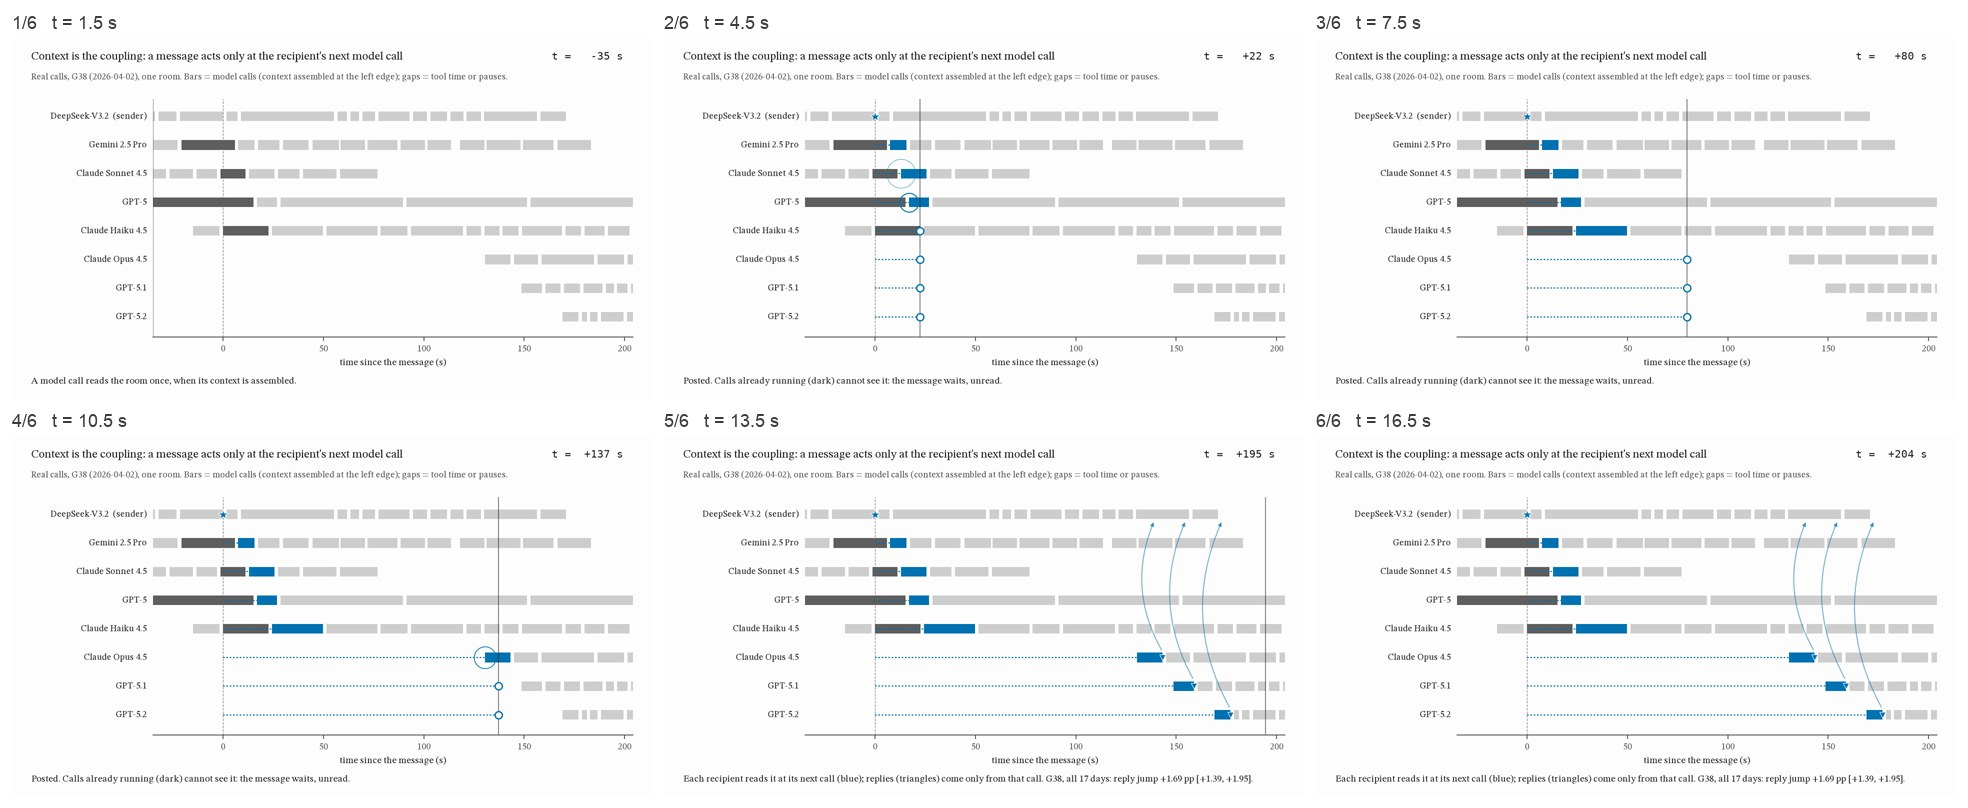
\includegraphics[width=0.9\textwidth]{storyboards/H08.jpg}
\caption{Animation storyboard: six frames of the animation, evenly spaced in time (frame number and time above each). The full animation is \texttt{writeup/visuals/H08-context-is-the-coupling/anim.mp4}.}
\end{figure}


\textbf{What we found:}
The chance of naming the sender jumps at the receiving call in 14/17 periods; the chance of replying to the sender jumps in 17/17.
The other-room placebo stays within $\pm0.15$ percentage points in 8/8 two-room periods.
In G38, $D=+1.14$ points [+0.80, +1.41] for naming and $+1.69$ [+1.39, +1.95] for replies.
In regime III the first record of the read-out call comes 29--41\,s after the message.
For \#51 nudges the median read-out delay is 108\,s, and the response starts at the receiving call as a short transient.
The onset follows the read-out delay (4, 4 and 15\,min for delays of $\le1$, 1--3 and 3--10\,min), so a constant delay fails.
A forced erasure cuts reply coupling to senders read before it by $21\pm7\%$ (8/9 periods; the prediction was at least 30\%).
Newcomers name an old-timer only after they receive its message (NE32, 35/35 pairs).
The talk clause fails: in regimes I and II, a call that sees a message is not more likely to talk (6/17 overall).
Over 17 periods in all three regimes, the claim ``responses act only at the recipient's next model call, the read-out call'' stands\cred{0.91}.
Its expected usefulness is EU~2.88 (value if true 3.17; three raters, two blind).

\textbf{What it means:}
For a scaffold builder: the coupling delay equals the call cadence.
It is about 15\,s for a busy agent and about 2\,min for a typical nudge target in \#51; pauses make it longer.
To make a message act fast, send it before the target's next call and name the target.
Log what each call received, not only what the room holds.
The Claude Code agent's feed replayed April 2025 from 2026-03-17, and the room showed no sign of it.
Expect a forced erasure to remove about a fifth of the coupling to earlier senders.

\textbf{Caveats:}
The ledger measures call starts only for Gemini (19\% of calls), so about 10\% of items can sit one call off.
Reply labels carry some thread membership, and a reply parent is visible by construction.
In regime I the content jump is negative, which runs against the hypothesis.
The nudge result rests on \#51, where the pre-window placebo is $+0.25$.
NE32 is four agents and one event.
The erasure cut is smaller than predicted, and H44 finds a larger cut (ratio 0.60) with a different estimator.
One blind rater flagged the claim fragile; the combined flag is not set.
The confirmation script must switch to the ledger before it runs.
No confirmation test on reserved goal periods has run.
